% All tables and figures for page 4.
% table* first so it spans both columns at the top of the page.
% Double-column floats (table*) must use [t]/[b]/[p]; [H] is single-column only.

\begin{table*}[t]
  \centering
  \footnotesize
  \caption{Representative SAE features of ViT-B/16. CLIP score: mean cosine similarity to the top-$K$ activating crops. RLD: mean relative logit drop under full ablation over the held-out evaluation set, with 95\% non-parametric bootstrap confidence interval. Acc: top-1 accuracy drop. Features labelled \emph{uncertain} fell within the per-layer CLIP abstention margin.}
  \label{tab:feature_results}
  \begin{tabular}{cllccc}
    \toprule
    Layer & Feature & CLIP concept & CLIP score & Mean RLD (\%) & 95\% CI (\%) \\
    \midrule
    2  & 2391 & uncertain (texture)             & 0.233 & $+0.082$ & $[+0.036,\,+0.129]$ \\
    \midrule
    9  & 2215 & Am.\ Staffordshire terrier      & 0.287 & $-0.084$ & $[-0.136,\,-0.036]$ \\
    9  & 5038 & red fox                         & 0.300 & $-0.027$ & $[-0.052,\,-0.005]$ \\
    \midrule
    10 & \textbf{1321} & \textbf{American lobster} & \textbf{0.310} & $\mathbf{+0.564}$ & $\mathbf{[+0.168,\,+1.037]}$ \\
    10 & 5609 & mortarboard                     & 0.323 & $+0.376$ & $[+0.060,\,+0.760]$ \\
    10 & 2723 & garden spider                   & 0.326 & $+0.172$ & $[+0.031,\,+0.356]$ \\
    \midrule
    11 & 3508 & meerkat                         & 0.308 & $+0.227$ & $[+0.037,\,+0.486]$ \\
    11 & 136  & mortarboard                     & 0.318 & $+0.152$ & $[-0.018,\,+0.369]$ \\
    11 & 596  & cauliflower                     & 0.335 & $+0.039$ & $[+0.000,\,+0.117]$ \\
    \bottomrule
  \end{tabular}
\end{table*}

\begin{table}[H]
  \centering
  \small
  \caption{ViT-B/16 SAE metrics and mean causal impact across depths. $\bar{L}_0$: avg.\ active features per patch token. Mean RLD reported over the held-out evaluation set with 95\% bootstrap CI.}
  \label{tab:layer_metrics}
  \begin{tabular}{lcccc}
    \toprule
    Layer & R\textsuperscript{2} & $\bar{L}_0$ & Mean RLD (\%) & 95\% CI (\%) \\
    \midrule
    2  (early) & 0.684 & 58.1 & $+0.032$ & $[+0.020,+0.045]$ \\
    9  (mid)   & 0.810 & 68.6 & $-0.019$ & $[-0.027,-0.012]$ \\
    10 (late)  & 0.866 & 40.8 & $+0.104$ & $[+0.047,+0.169]$ \\
    11 (late)  & 0.890 & 29.0 & $+0.078$ & $[+0.049,+0.112]$ \\
    \bottomrule
  \end{tabular}
\end{table}

\begin{table}[H]
  \centering
  \small
  \caption{Causal ablation controls on ViT-B/16 (same evaluation split, same number of ablated units as the SAE-feature condition).}
  \label{tab:causal_controls}
  \begin{tabular}{lcccc}
    \toprule
    Layer & SAE features RLD (\%) & Random dirs RLD (\%) & Dead features RLD (\%) & Raw neurons RLD (\%) \\
    \midrule
    2  & $+0.032$ & $+0.005$ [$-0.020,+0.030$] & $+0.001$ [$-0.002,+0.004$] & $+0.020$ [$-0.040,+0.080$] \\
    9  & $-0.019$ & $-0.002$ [$-0.025,+0.020$] & $+0.000$ [$-0.001,+0.001$] & $-0.010$ [$-0.060,+0.045$] \\
    10 & $+0.104$ & $+0.008$ [$-0.025,+0.040$] & $+0.001$ [$-0.002,+0.003$] & $+0.050$ [$-0.070,+0.150$] \\
    11 & $+0.078$ & $+0.006$ [$-0.018,+0.032$] & $+0.000$ [$-0.001,+0.002$] & $+0.045$ [$-0.060,+0.120$] \\
    \bottomrule
  \end{tabular}
\end{table}

\begin{table}[H]
  \centering
  \small
  \caption{Supervised ViT-B/16 vs.\ self-supervised DINOv2-B under an \emph{identical} SAE recipe (expansion $8$, $20$ epochs, per-layer $\lambda$). DINOv2 attains $99.5\%$ linear-probe accuracy yet its dictionaries collapse to dead latents ($\bar{L}_0\!\to\!0$) at every depth except the mid-network Layer~9.}
  \label{tab:backbone_compare}
  \begin{tabular}{lcccc}
    \toprule
    & \multicolumn{2}{c}{ViT-B/16} & \multicolumn{2}{c}{DINOv2-B} \\
    \cmidrule(lr){2-3}\cmidrule(lr){4-5}
    Layer & R\textsuperscript{2} & $\bar{L}_0$ & R\textsuperscript{2} & $\bar{L}_0$ \\
    \midrule
    2  & 0.684 & 58.1 & 0.087  & 0.86 \\
    9  & 0.810 & 68.6 & 0.843  & 0.07 \\
    10 & 0.866 & 40.8 & 0.089  & 0.02 \\
    11 & 0.890 & 29.0 & $-0.006$ & 0.00 \\
    \bottomrule
  \end{tabular}
\end{table}

\begin{figure}[H]
  \centering
  \begin{minipage}{0.48\columnwidth}
    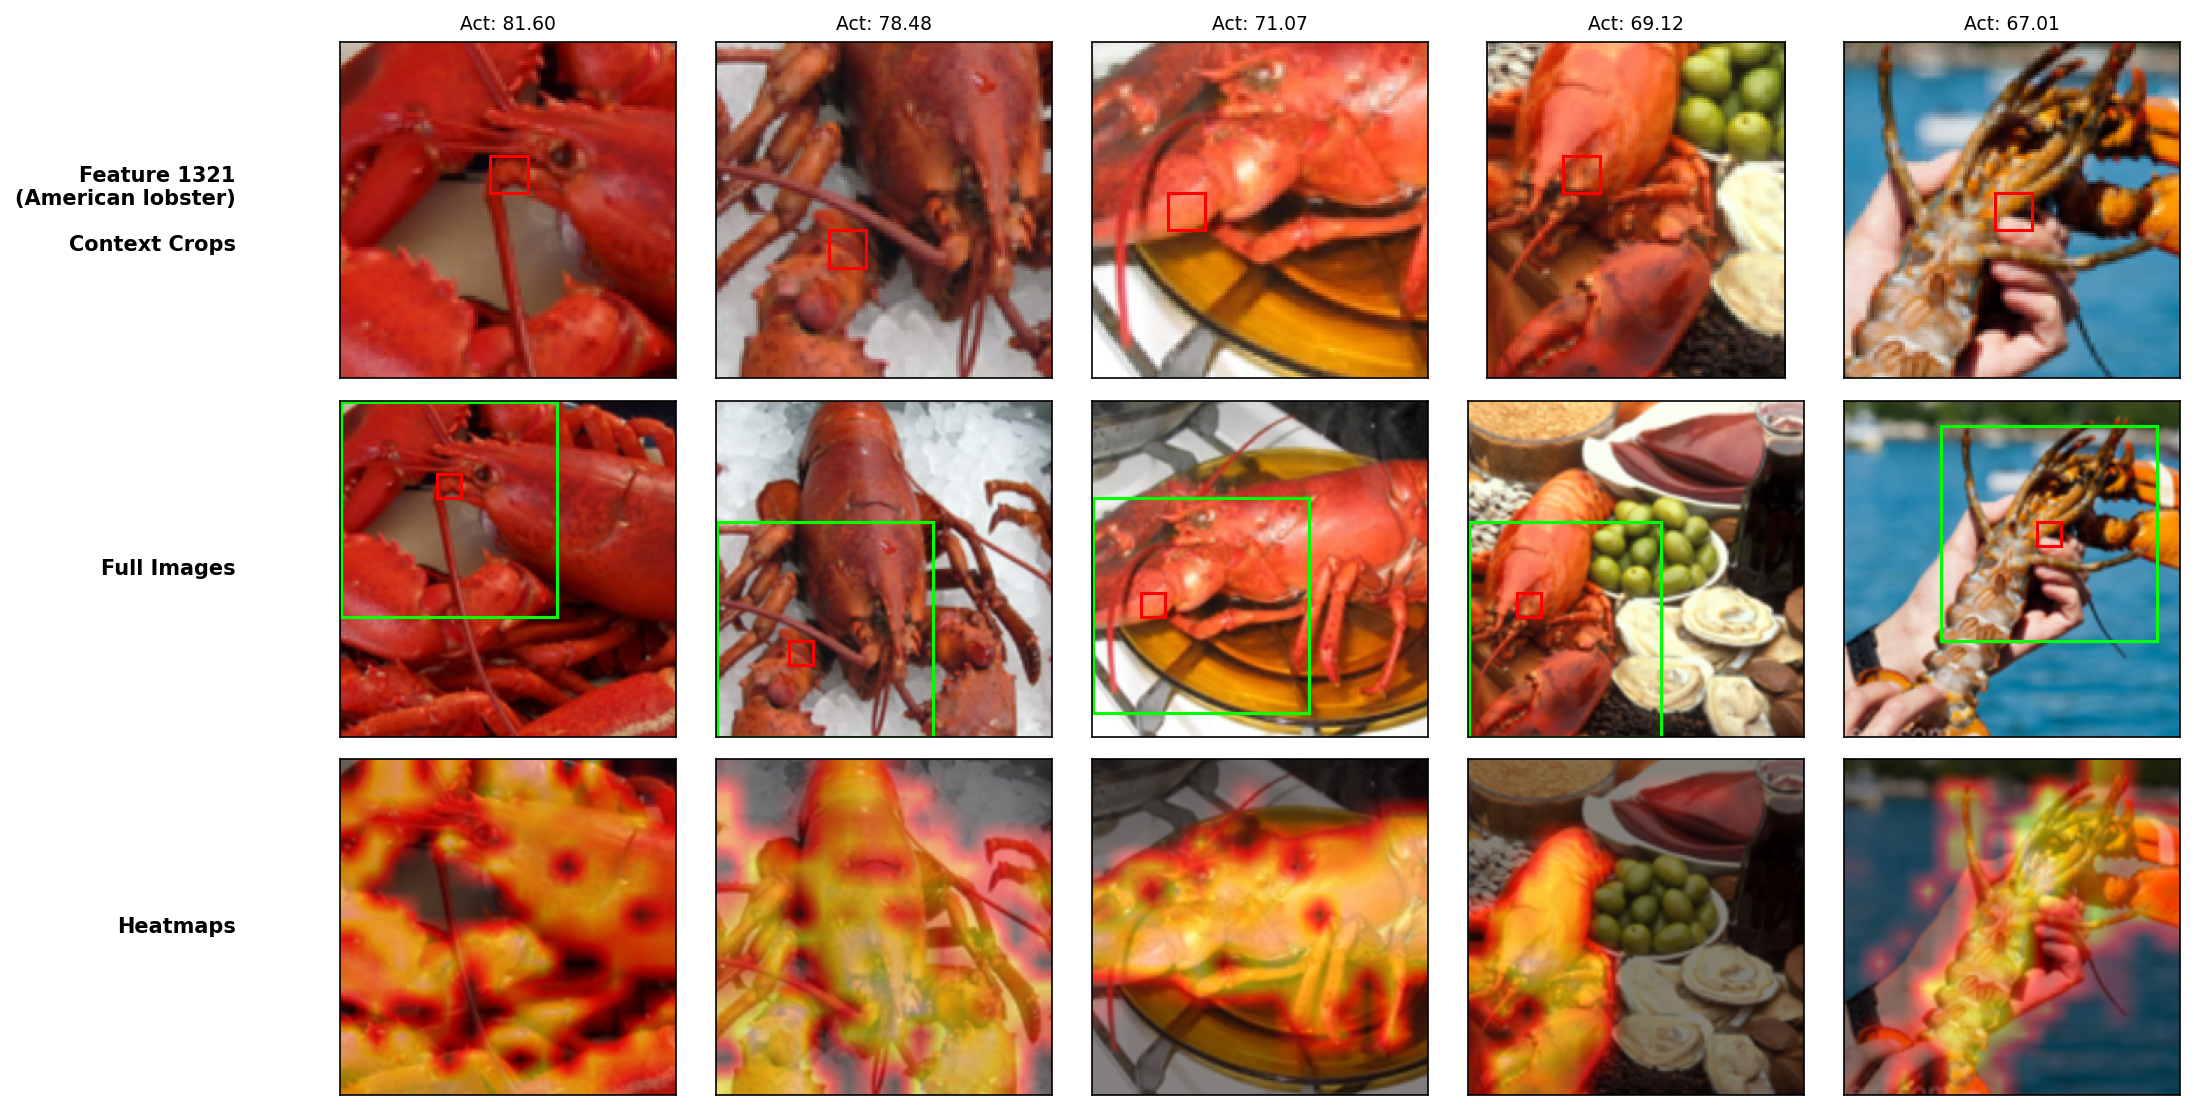
\includegraphics[width=\linewidth]{Figures/vit_grid_lobster.png}
  \end{minipage}\hfill
  \begin{minipage}{0.48\columnwidth}
    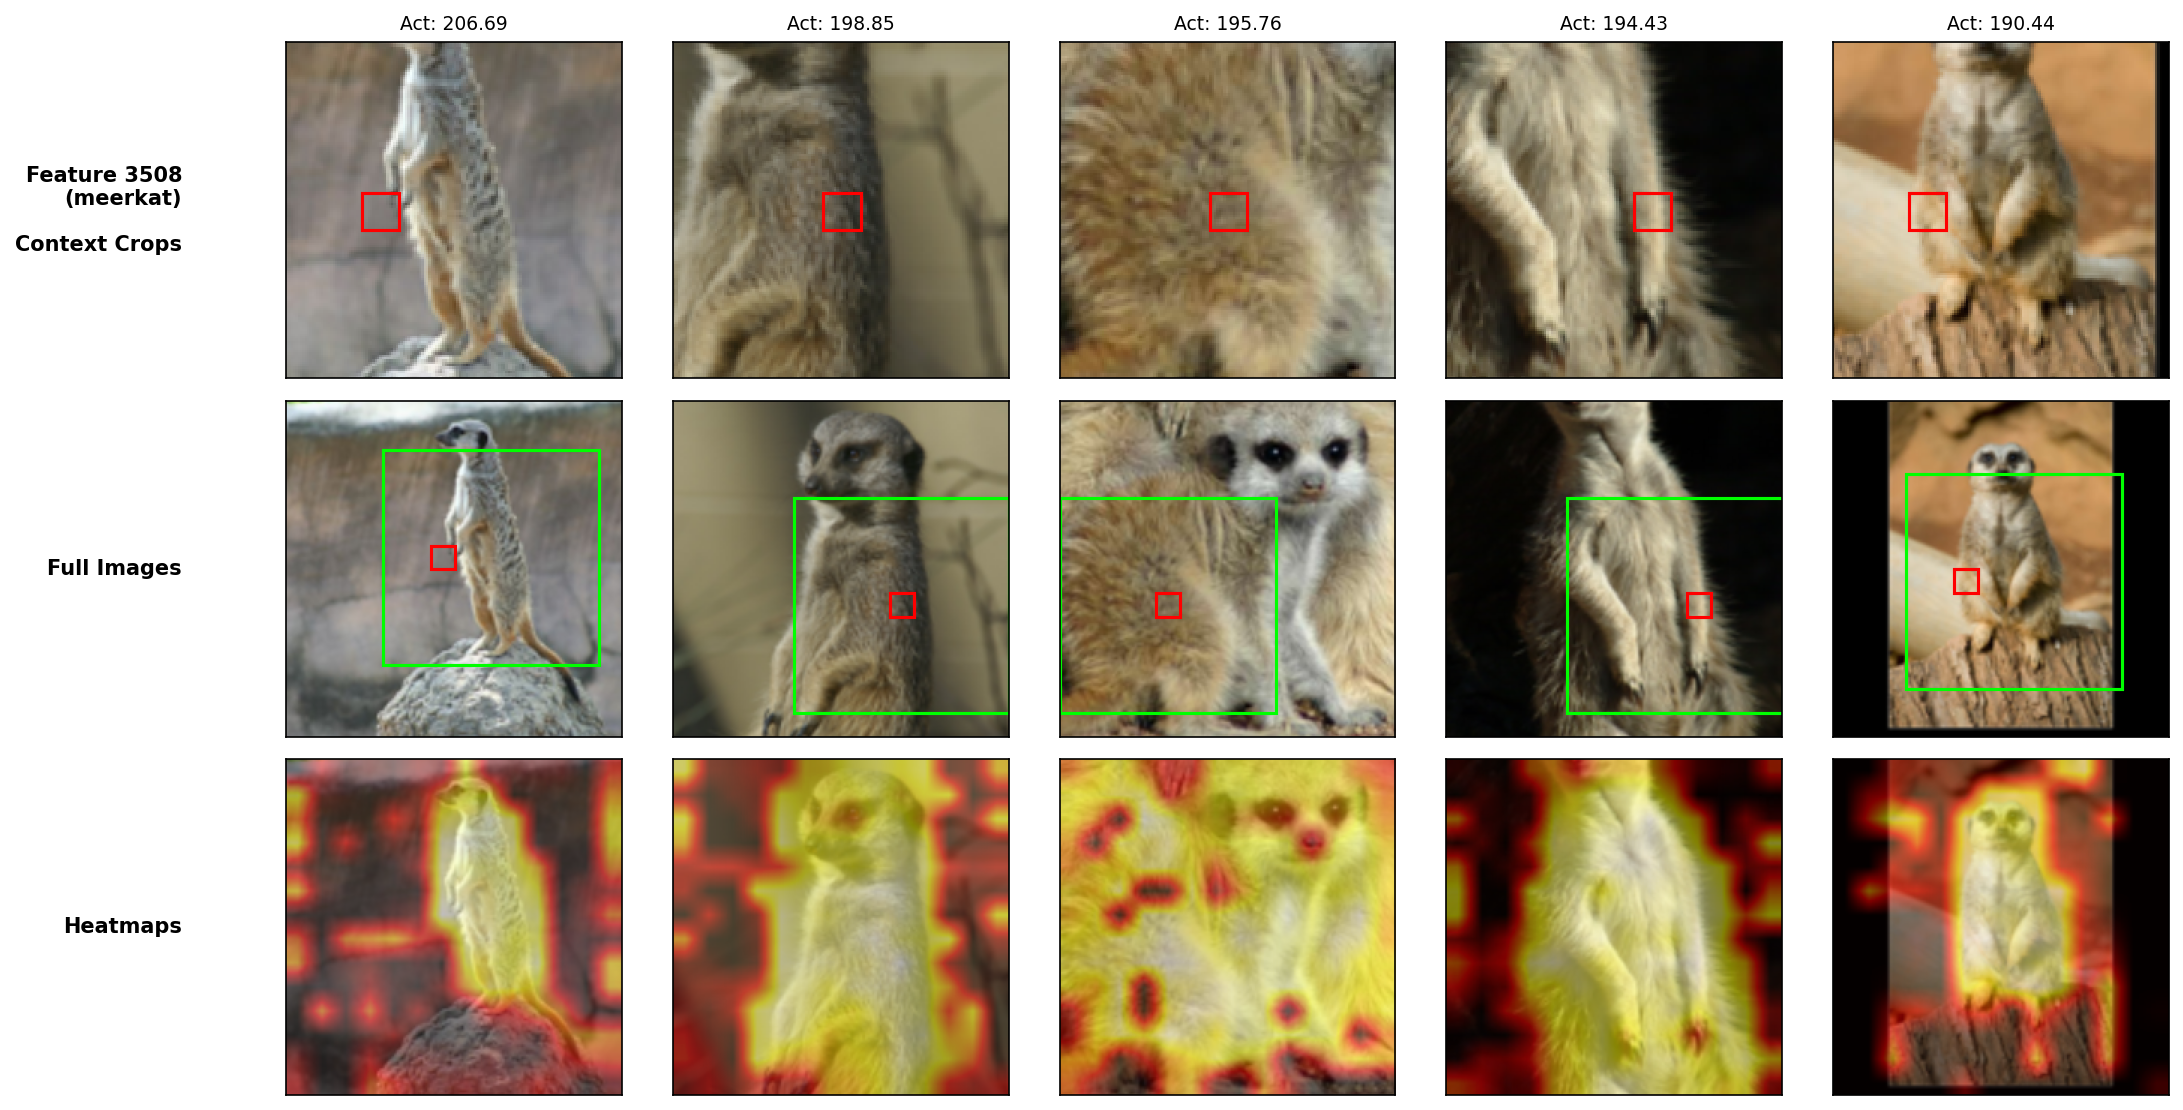
\includegraphics[width=\linewidth]{Figures/vit_grid_meerkat.png}
  \end{minipage}
  \caption{Two monosemantic late-layer ViT features. Left: \textit{American lobster} (Feature~1321, Layer~10), the most causal feature ($+0.564\%$ RLD). Right: \textit{meerkat} (Feature~3508, Layer~11). Each block shows activation-guided crops, full images with the peak patch (red) and activation region (green), and activation heatmaps. Heatmaps concentrate on the object, not the background.}
  \label{fig:grid_semantic}
\end{figure}

\begin{figure}[H]
  \centering
  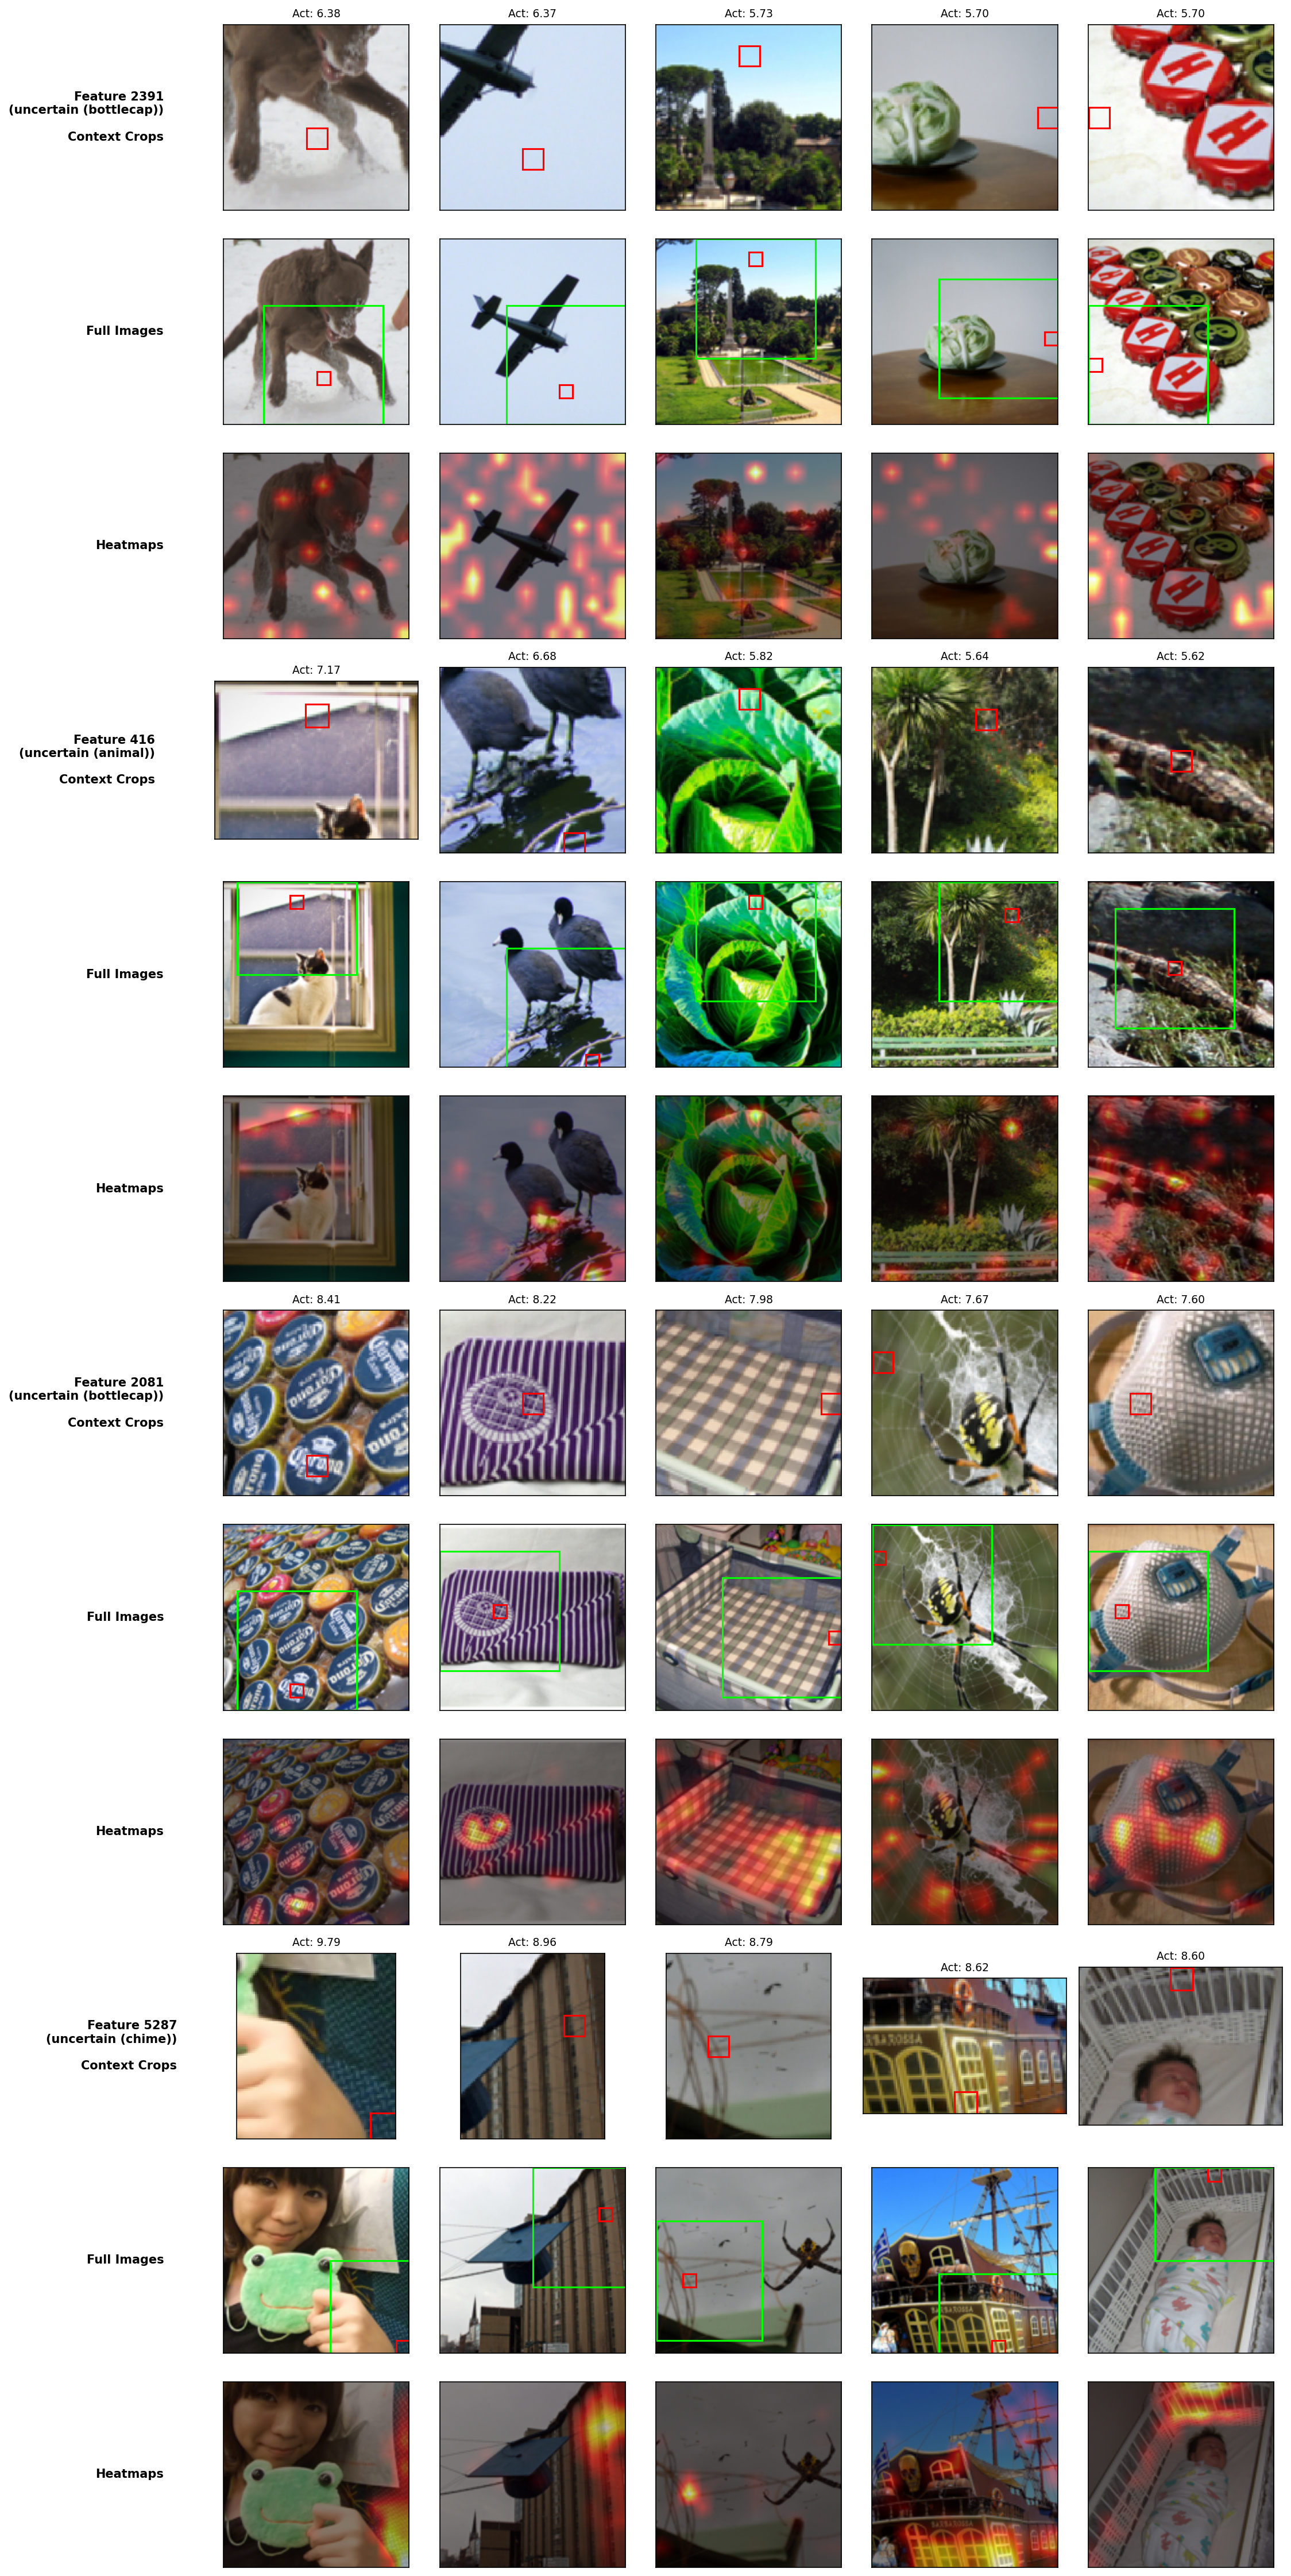
\includegraphics[width=0.85\columnwidth, trim=0 1680px 0 0, clip]{Figures/vit_multilayer_layer2.png}
  \caption{Early-layer (Layer~2) ViT features. All ten top features fall below the CLIP abstention margin (\emph{uncertain}); the exemplars and heatmaps reveal low-level texture and local-structure detectors rather than object concepts, consistent with the role of early MLP layers \cite{Raghu2021}.}
  \label{fig:grid_early}
\end{figure}

\begin{figure}[H]
  \centering
  \begin{minipage}{0.95\columnwidth}
    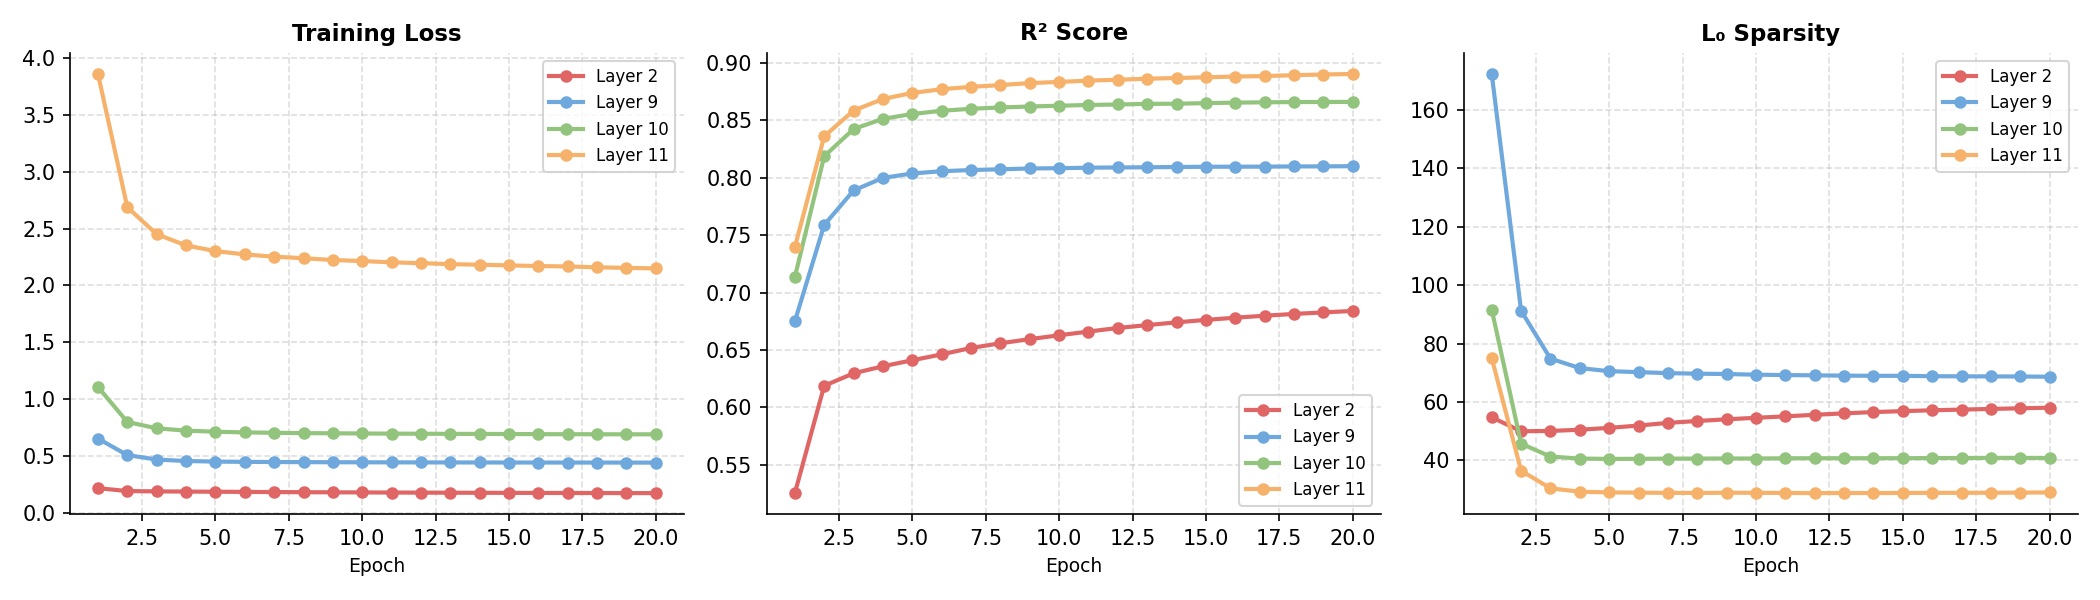
\includegraphics[width=\linewidth]{Figures/vit_training_curves.png}
  \end{minipage}

  \vspace{0.5em}

  \begin{minipage}{0.95\columnwidth}
    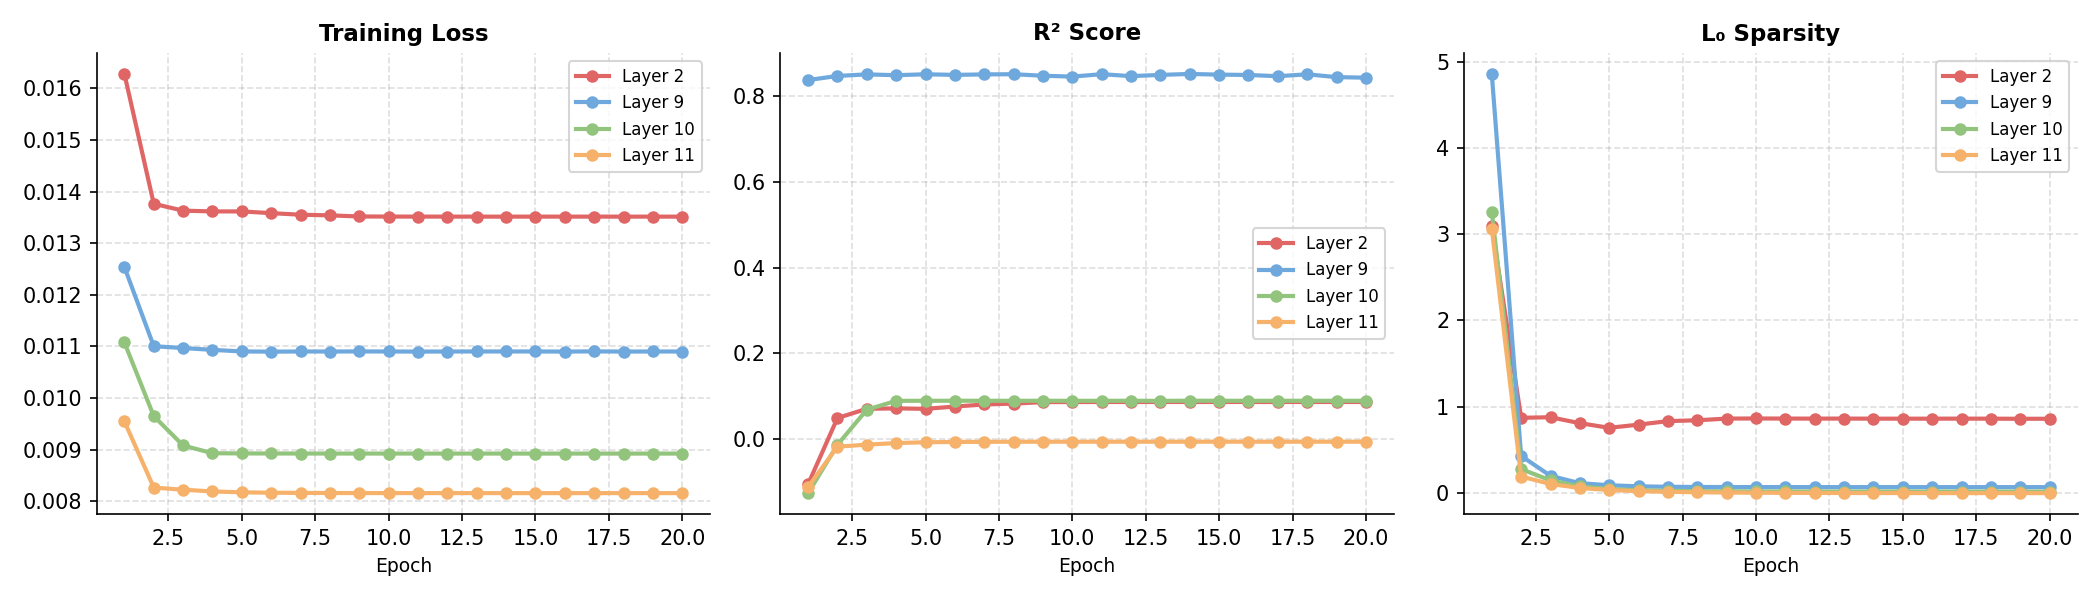
\includegraphics[width=\linewidth]{Figures/dino_training_curves.png}
  \end{minipage}
  \caption{SAE training convergence. Top: ViT-B/16 (Layers~2/9/10/11) converges stably to $R^2$ between $0.68$ and $0.89$ with non-trivial sparsity. Bottom: DINOv2-B under the identical recipe---only Layer~9 trains to a high $R^2$, while Layers~2/10/11 collapse ($\bar{L}_0\!\to\!0$, $R^2\!\le\!0.09$), the signature of an over-sparsified, dead dictionary.}
  \label{fig:training_curves}
\end{figure}

\begin{figure}[H]
  \centering
  \begin{minipage}{0.48\columnwidth}
    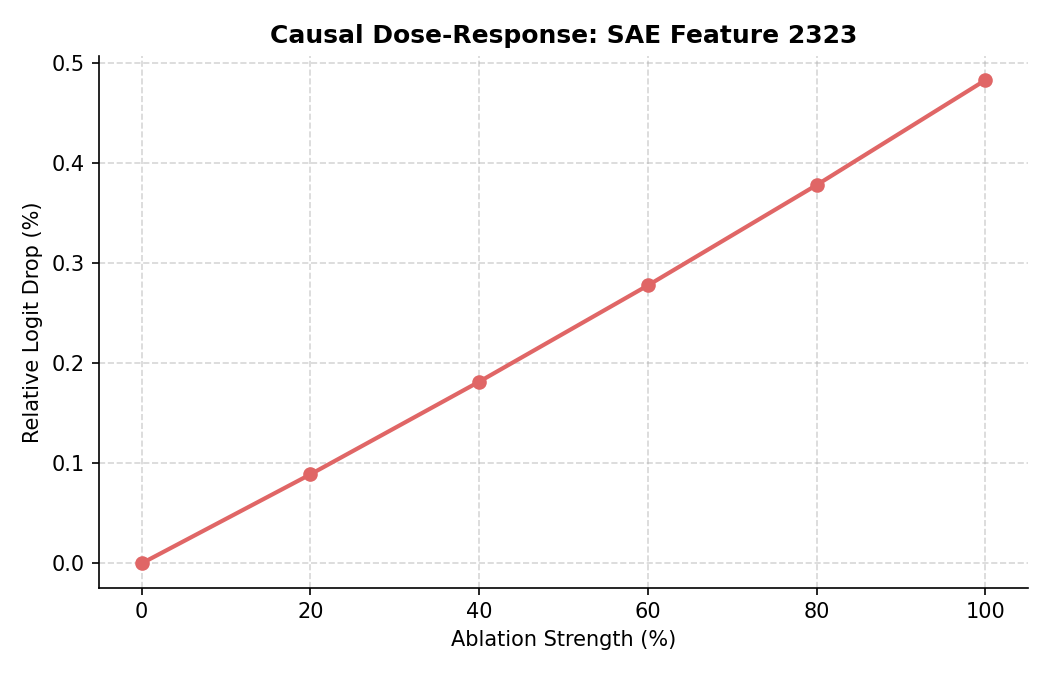
\includegraphics[width=\linewidth]{Figures/vit_dose_response.png}
  \end{minipage}\hfill
  \begin{minipage}{0.48\columnwidth}
    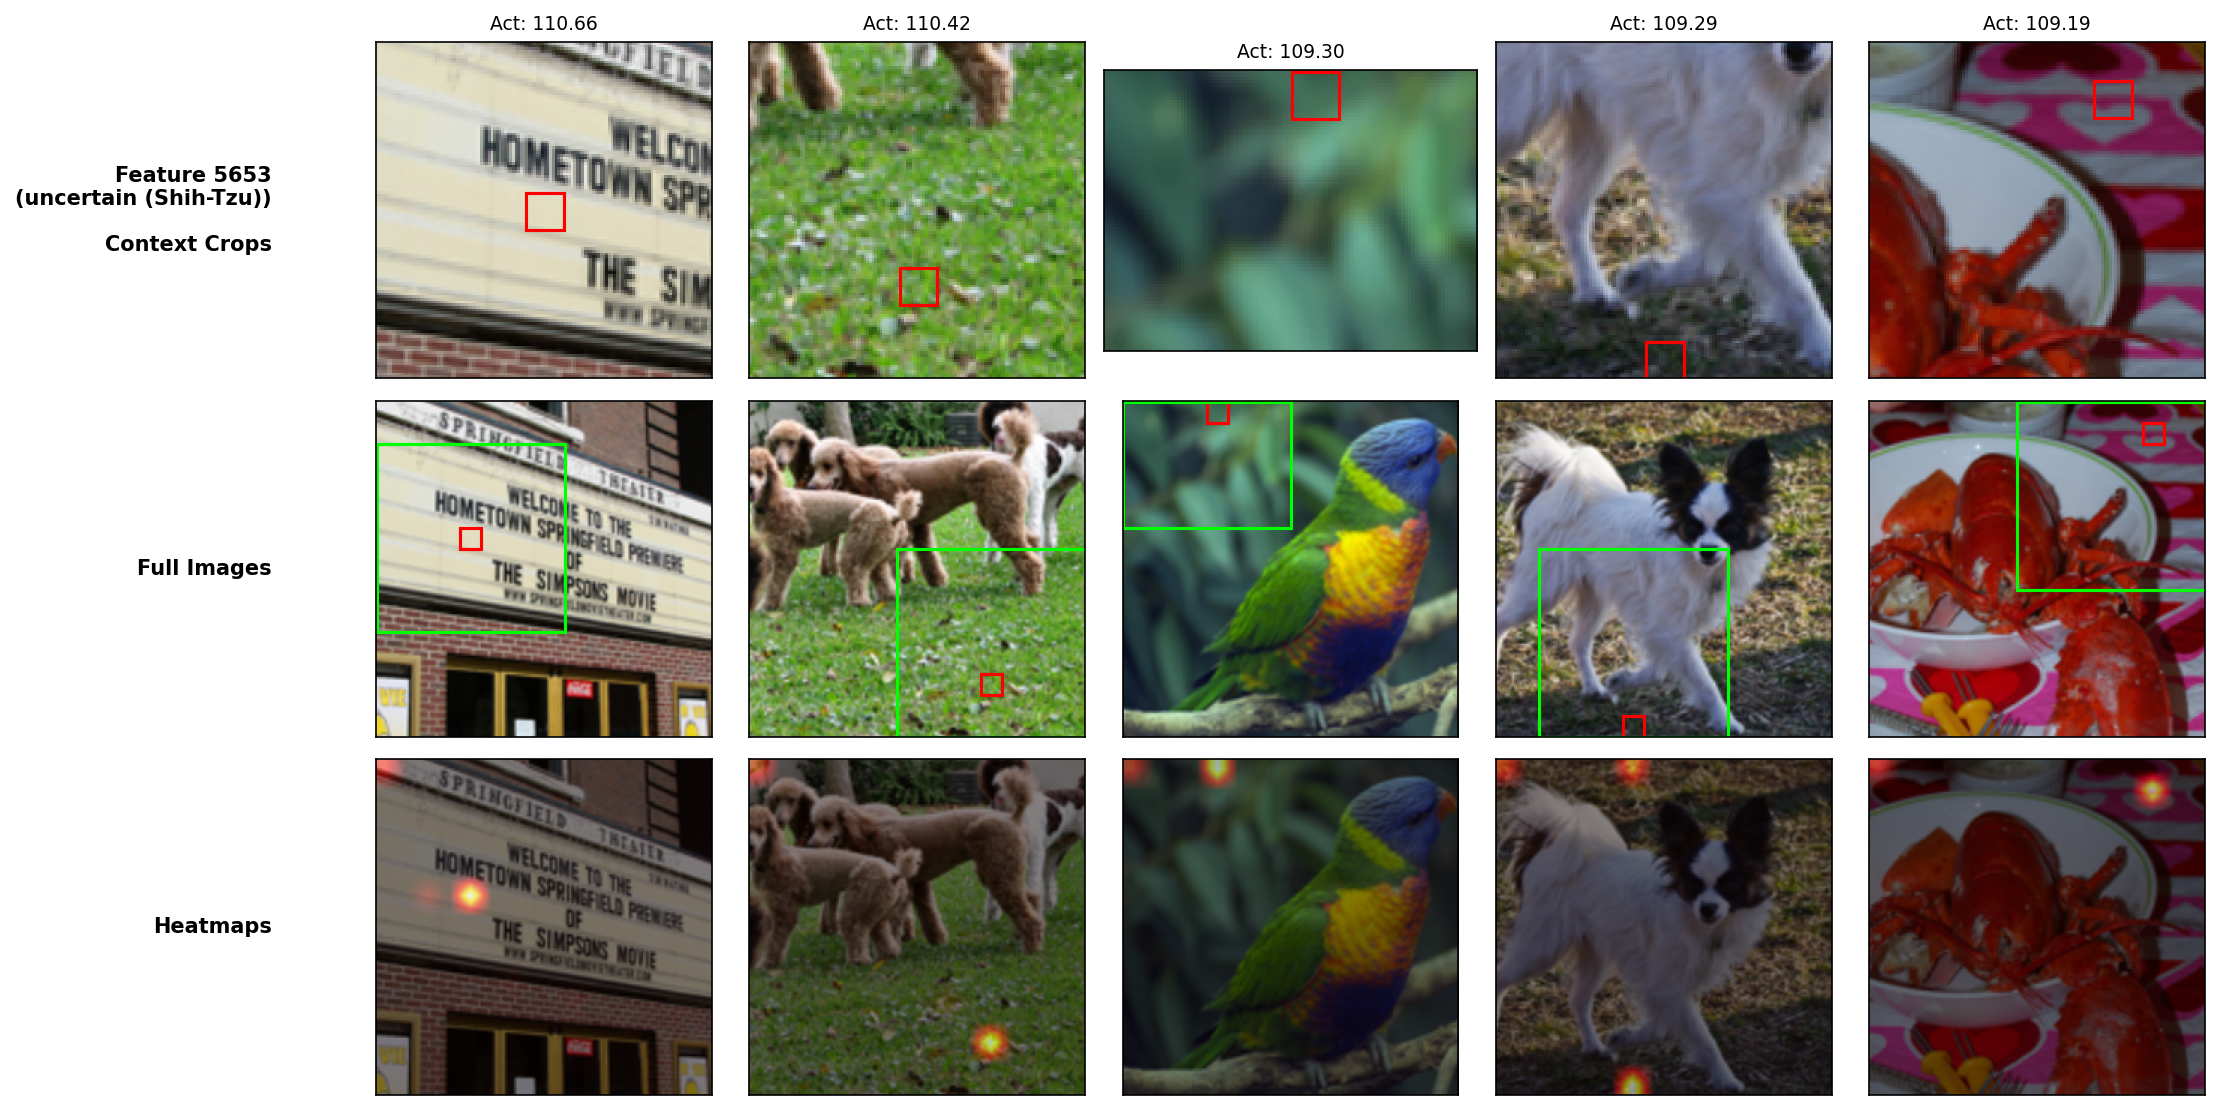
\includegraphics[width=\linewidth]{Figures/dino_grid_layer9.png}
  \end{minipage}
  \caption{Left: dose-response curve for the strongest late-layer ViT feature---logit drop increases monotonically with ablation strength $s\!\in\![0,1]$, ruling out an artefactual causal signal. Right: the only causal DINOv2 feature (Layer~9, Feature~5653); although causal ($+0.60\%$ RLD), its exemplars (marquee, poodles, parrot, lobster) are visibly polysemantic, illustrating why matched-recipe SAEs yield poorly separated features on the self-supervised backbone.}
  \label{fig:causal}
\end{figure}
